\documentclass[10pt,a4paper]{article}
\usepackage[T1]{fontenc}
\usepackage{tgtermes}
\usepackage{moresize}
\usepackage[utf8]{inputenc}
\usepackage{graphicx}
\usepackage{xcolor}
\usepackage[a4paper, total={200mm, 285mm}]{geometry}
\usepackage{float}
\usepackage{indentfirst}
\usepackage{multicol}
\usepackage[font=tiny]{caption}
\usepackage{graphics}
\usepackage{listings}
\usepackage{amsmath} 
% \usepackage[norsk]{babel}
\usepackage{comment}
\usepackage{tikz}
\usetikzlibrary{arrows.meta,positioning}

% TODO: 
% - legge til reverse BWT, MFT
% - Skrive mer om dekompremering av algoritmene 
% - flere bilder, diagrammer og tabeller IN PROGRESS
% - pros/cons analyse for sorteringsalgo DONE
% - Prioritetskø: kompleksitet for operasjoner DONE 
% - Eksempler på kompleksitetanalyse IN PROGRESS
% - TRENGER CLAUD!!!! Token limit 
% - Flere eksamensoppgaver eksempler IN PROGRESS

% \usepackage{draftwatermark}
% \SetWatermarkText{linkedin.com/in/tritacle}
% \SetWatermarkScale{0.6}

% Moderne fargepalett
\definecolor{primaryblue}{RGB}{25, 60, 110}      % Hovedoverskrifter
\definecolor{accentteal}{RGB}{0, 120, 120}       % Underoverskrifter
\definecolor{warmamber}{RGB}{180, 100, 0}        
\definecolor{codebackground}{RGB}{245, 245, 245}
\definecolor{mGreen}{RGB}{0, 128, 0}
\definecolor{mPurple}{RGB}{128, 0, 128}
\definecolor{mGray}{RGB}{128, 128, 128}


\usepackage{setspace}

% Rett før \begin{document}
\setlength{\parskip}{0pt}
\setlength{\parindent}{0pt}
\renewcommand{\baselinestretch}{1.0}
\begin{document}
\begin{multicols}{4}
{\fontsize{8}{8}\selectfont
\setlength{\baselineskip}{8pt}  
\setlength{\parskip}{0pt}
\setlength{\lineskip}{0pt}
\setlength{\lineskiplimit}{0pt}
\linespread{1.0}                
\noindent
\textcolor{primaryblue}{\textbf{Tidskompleksitet}}\textcolor{black}: 
$O$ øvre grense. $\Omega$ nedre grense. $\Theta$ øvre og nedre grense, om de er like. Noen regler:
\noindent
\vspace{-7pt}
\begin{lstlisting}[
    backgroundcolor=\color{white},   
    commentstyle=\color{mGreen},
    keywordstyle=\color{magenta},
    numberstyle=\tiny\color{mGray},
    stringstyle=\color{mPurple},
    basicstyle=\footnotesize,
    breakatwhitespace=false,         
    breaklines=true,                 
    captionpos=b,                    
    keepspaces=true,                 
    numbers=left,                    
    numbersep=5pt,                  
    showspaces=false,                
    showstringspaces=false,
    showtabs=false,                  
    tabsize=2,
    language=C,
    basicstyle=\fontsize{6.3}{8}\selectfont,
    mathescape=true
]
for (i=0; i<n; i+=k); // $\Theta(n/k)$
for (i=1; i<n; i*=k); // $\Theta(log_k n)$
for (i=0; i<n/k; i++); // $\Theta(n/k)$
for (i=j; i>0; i/=k); // $\Theta(log_k j)$
for (i=j; i>n; i/=k); // $\Theta(log(j/n))$
for (i=0; i<n; i++){
    for (j=i; j<n; j++);} // $\Theta(n^2)$ 
for (i=0; i<n; i++){
    for (j=0; j<i; j++)} // $\Theta(n^2)$ 
for (i=a; i<b; i++) // $\Theta(b-a)$
for (i=a; i<b; i+=c) // $\Theta((b-a)/c)$
\end{lstlisting}
\vspace{-5pt}
\noindent
\includegraphics[width=4.7cm]{images/mestermetoden.png}
\\
\noindent
\textcolor{accentteal}{\textbf{Eksempler}}\textcolor{black}: 
\noindent 
Lineær rekursjon, $\mathbf{\Theta(n)}$
\begin{lstlisting}[
    backgroundcolor=\color{white},   
    commentstyle=\color{mGreen},
    keywordstyle=\color{magenta},
    numberstyle=\tiny\color{mGray},
    stringstyle=\color{mPurple},
    basicstyle=\footnotesize,
    breakatwhitespace=false,         
    breaklines=true,                 
    captionpos=b,                    
    keepspaces=true,                 
    numbers=left,                    
    numbersep=5pt,                  
    showspaces=false,                
    showstringspaces=false,
    showtabs=false,                  
    tabsize=2,
    language=C,
    basicstyle=\fontsize{7}{8}\selectfont,
    mathescape=true
]
func1(n, x) {
    if (n == 0) return 1;
    else return x * func(n-1, x)
}
\end{lstlisting}
\vspace{-5pt}

\noindent
Rekursjon med $n/2$, $\mathbf{\Theta(\log n)}$
\begin{lstlisting}[
    backgroundcolor=\color{white},   
    commentstyle=\color{mGreen},
    keywordstyle=\color{magenta},
    numberstyle=\tiny\color{mGray},
    stringstyle=\color{mPurple},
    basicstyle=\footnotesize,
    breakatwhitespace=false,         
    breaklines=true,                 
    captionpos=b,                    
    keepspaces=true,                 
    numbers=left,                    
    numbersep=5pt,                  
    showspaces=false,                
    showstringspaces=false,
    showtabs=false,                  
    tabsize=2,
    language=C,
    basicstyle=\fontsize{6.5}{8}\selectfont,
    mathescape=true
]
func2(int n, float x) {
    if (n == 0) return 1.0;
    else return x * prog_d(n/2, x)
}
\end{lstlisting}
\vspace{-5pt}

\noindent
$A$ rekursive kall med $n/3$ hver. $A$ er konstant,  $T(n) = A \cdot T(n/3) + c \cdot n^0$. Her: $a=A, b=3, k=0$. $b^k = 3^0 = 1 < A$ $\to$ tilfelle 1 $\to$ $\mathbf{\Theta(n^{\log_3 A})}$
\begin{lstlisting}[
    backgroundcolor=\color{white},   
    commentstyle=\color{mGreen},
    keywordstyle=\color{magenta},
    numberstyle=\tiny\color{mGray},
    stringstyle=\color{mPurple},
    basicstyle=\footnotesize,
    breakatwhitespace=false,         
    breaklines=true,                 
    captionpos=b,                    
    keepspaces=true,                 
    numbers=left,                    
    numbersep=5pt,                  
    showspaces=false,                
    showstringspaces=false,
    showtabs=false,                  
    tabsize=2,
    language=C,
    basicstyle=\fontsize{6}{8}\selectfont,
    mathescape=true
]
func3(n, t) {
    if (n > 0) {
        for(int i = 1; i <= A; ++i){
            tri += prog_f(n/3);
        }
        return t;
    } else return -1;
}
\end{lstlisting}
\vspace{-5pt}

\noindent
To rekursive kall med $(n/2, q/4)$ + løkke over $q$. . Kompleksiteten avhenger av $q$, ikke $n$! For $q$: $a=2, b=4, k=1$. $b^k = 4^1 = 4 > 2$ $\to$ tilfelle 3 $\to$ $\mathbf{O(q^1) = O(q)}$ ikke $O(n)$!
\begin{lstlisting}[
    backgroundcolor=\color{white},   
    commentstyle=\color{mGreen},
    keywordstyle=\color{magenta},
    numberstyle=\tiny\color{mGray},
    stringstyle=\color{mPurple},
    basicstyle=\footnotesize,
    breakatwhitespace=false,         
    breaklines=true,                 
    captionpos=b,                    
    keepspaces=true,                 
    numbers=left,                    
    numbersep=5pt,                  
    showspaces=false,                
    showstringspaces=false,
    showtabs=false,                  
    tabsize=2,
    language=C,
    basicstyle=\fontsize{6.5}{8}\selectfont,
    mathescape=true
]
func4(q, n, [] t) {
    int sum = 0;
    if (q > 0) {
       sum += prog_c(n/2, q/4, t);
       for (int i=0; i<q; ++i)
            sum += t[i*n+q];
       sum += prog_c(n/2, q/4, t);
    }
    return sum;
}
\end{lstlisting}
\vspace{-5pt}

\noindent
Dobbel løkke $a \cdot b$ + enkel løkke $b$. $\mathbf{\Theta(ab+a+b)}$. Alternativt: $\Theta(ab)$ når $a,b>0$, $\Theta(b)$ når $a=0$, $\Theta(a)$ når $b=0$.
\begin{lstlisting}[
    backgroundcolor=\color{white},   
    commentstyle=\color{mGreen},
    keywordstyle=\color{magenta},
    numberstyle=\tiny\color{mGray},
    stringstyle=\color{mPurple},
    basicstyle=\footnotesize,
    breakatwhitespace=false,         
    breaklines=true,                 
    captionpos=b,                    
    keepspaces=true,                 
    numbers=left,                    
    numbersep=5pt,                  
    showspaces=false,                
    showstringspaces=false,
    showtabs=false,                  
    tabsize=2,
    language=C,
    basicstyle=\fontsize{7}{8}\selectfont,
    mathescape=true
]
func5(a, b) {
    int sum = 0;
    for (int i=0; i<a ; ++i){
       for (int j=0; j<b; ++j){
            sum += i*j; 
        }
    }
    for (int k=0; k < b; ++k){
        sum += k; 
    }
    return sum; 
}
\end{lstlisting}
\vspace{-5pt}
\noindent
\textcolor{primaryblue}{\textbf{Rekursjon:}} \color{black} Bruker \textit{mestermetoden} for å finne tidskompleksitet til rekursive algoritmer. $T(n) = a \cdot T(n/b) + cn^k$. $a$: antall rekursive kall, $b$: brøkdelen av datasetter vi behandler i et rekursivt kall. $cn^k$: kompleksitet utenfor rekursjonen. 
\newline 1. $b^k < a \rightarrow T(n) \in \Theta (n^{log_b a})$
\newline 2. $b^k = a \rightarrow T(n) \in \Theta (n^k \cdot log(n))$
\newline 3. $b^k > a \rightarrow T(n) \in \Theta (n^k)$
\vspace{-7pt}
\begin{lstlisting}[
    backgroundcolor=\color{white},   
    commentstyle=\color{mGreen},
    keywordstyle=\color{magenta},
    numberstyle=\tiny\color{mGray},
    stringstyle=\color{mPurple},
    basicstyle=\footnotesize,
    breakatwhitespace=false,         
    breaklines=true,                 
    captionpos=b,                    
    keepspaces=true,                 
    numbers=left,                    
    numbersep=5pt,                  
    showspaces=false,                
    showstringspaces=false,
    showtabs=false,                  
    tabsize=2,
    language=java,
    basicstyle=\fontsize{5}{8}\selectfont
]
sum(int[] arr, int l, int r) {
    int m = (l + r) / 2;
    return sum(arr, l, m) + sum(arr, m+1, r)
}
\end{lstlisting}
\vspace{-7pt}
\noindent
$T(n) = 2 \cdot T(n/2) + c \cdot n^0$
$T(n) = \Theta(n^{log_22}) = \Theta(n)$
\newline
\noindent
\textcolor{primaryblue}{\textbf{Lineær rekursjon:}}
\noindent Hvis rekursjonsvariabelen minker med $(n - 1)$ (antar $a=1$) får vi $T(n-1) + cn^k \in \Theta(n + cn^k)$
\newline
\textcolor{primaryblue}{\textbf{---Sorteringsalgoritmer---}}
\newline
\textcolor{accentteal}{\textbf{Innsetting-:}}
\vspace{-7pt}
\begin{lstlisting}[
    backgroundcolor=\color{white},   
    commentstyle=\color{mGreen},
    keywordstyle=\color{magenta},
    numberstyle=\tiny\color{mGray},
    stringstyle=\color{mPurple},
    basicstyle=\footnotesize,
    breakatwhitespace=false,         
    breaklines=true,                 
    captionpos=b,                    
    keepspaces=true,                 
    numbers=left,                    
    numbersep=5pt,                  
    showspaces=false,                
    showstringspaces=false,
    showtabs=false,                  
    tabsize=2,
    language=java,
    basicstyle=\fontsize{4.5}{8}\selectfont
]
innsettingssort([]arr){
    for (i = 1; i < arr.length; i++) {
        key = arr[i];
        j = i - 1;
        while (j >= 0 && arr[j] > key) {
            arr[j+1] = arr[j];  // Flytt bakover
            j--;
        }
        arr[j+1] = key;  // Sett inn paa riktig plass
    }
}
\end{lstlisting}
\vspace{-5pt}
Går gjennom arrayet element for element. \hspace{-3pt}For hvert element, flytt det bakover til riktig sortert posisjon blant de allerede sorterte elementene. \textit{Pros:} Rask for små datasett eller delvis sorterte data: $\Omega(n)$. \textit{Cons:} Treg på store, usorterte datasett: $O(n^2)$ om betingelsen slår til hver gang. Mye flytting av data.
\noindent \textcolor{accentteal}{\textbf{Boble-:}}
\vspace{-7pt}
\begin{lstlisting}[
    backgroundcolor=\color{white},   
    commentstyle=\color{mGreen},
    keywordstyle=\color{magenta},
    numberstyle=\tiny\color{mGray},
    stringstyle=\color{mPurple},
    basicstyle=\footnotesize,
    breakatwhitespace=false,         
    breaklines=true,                 
    captionpos=b,                    
    keepspaces=true,                 
    numbers=left,                    
    numbersep=5pt,                  
    showspaces=false,                
    showstringspaces=false,
    showtabs=false,                  
    tabsize=2,
    language=java,
    basicstyle=\fontsize{6.3}{8}\selectfont
]
boblesort([]arr){
    for (i = 0; i < arr.length; i++) {
        for (j = 0; j < i; j++) {
            if (arr[j] > arr[j+1]) {
                bytt(arr, j, j+1)
            }
        }
    }
}
\end{lstlisting}
\vspace{-5pt}
Går gjennom arrayet $n-1$ ganger. \hspace{-2pt}Hver iterasjon, sammenlignes naboelementer og byttes hvis de er i feil rekkefølge. Største tallet "synker" til sisteplass i tabellen i første iterasjon, mens små tall "bobler" opp. I neste iterasjon er det ikke nødvendig å ta med det siste tallet, så hver iterasjon blir ett tall kortere. Treg på store datasett. Mange sammenligninger og bytter selv på nesten sorterte data. $\mathbf{\Theta(n^2)}$.

\noindent \textcolor{accentteal}{\textbf{Velge-:}}
\vspace{-7pt}
\begin{lstlisting}[
    backgroundcolor=\color{white},   
    commentstyle=\color{mGreen},
    keywordstyle=\color{magenta},
    numberstyle=\tiny\color{mGray},
    stringstyle=\color{mPurple},
    basicstyle=\footnotesize,
    breakatwhitespace=false,         
    breaklines=true,                 
    captionpos=b,                    
    keepspaces=true,                 
    numbers=left,                    
    numbersep=5pt,                  
    showspaces=false,                
    showstringspaces=false,
    showtabs=false,                  
    tabsize=2,
    language=java,
    basicstyle=\fontsize{4.5}{8}\selectfont
]
velgesort(int[] arr){
	for (int i = 0; i < arr.length - 1; i--){
		int maxIdx = 0;
		for (int j=1; j <= i; j++){
			if (arr[j] > tall[maxIdx]){
				maxIdx = j
			}
		}
		if (maxIdx!=i) bytt(arr, i, maxIdx);
	}
}
\end{lstlisting}
\vspace{-5pt}
Finn største verdi, bytt den inn på plass $n-1$. Bytt nest største inn på plass $n-2$. Fortsett slik til vi har byttet nest minste inn på plass $1$. Gjør like mange sammenlikninger som boblesortering, men færre ombyttinger. Velgesortering bytter om tall maksimalt én gang for hvert iterasjon av den ytre løkka. $\mathbf{\Theta(n^2)}$
\noindent \textcolor{accentteal}{\textbf{Kvadratiske sorteringsalgoritmer:}} Sortere ved å bytte nabotall (algo ovenfor) er $\mathbf{\Omega(n^2)}$.
\noindent \textcolor{accentteal}{\textbf{Shell-}}
\vspace{-13pt}
\begin{lstlisting}[
    backgroundcolor=\color{white},   
    commentstyle=\color{mGreen},
    keywordstyle=\color{magenta},
    numberstyle=\tiny\color{mGray},
    stringstyle=\color{mPurple},
    basicstyle=\footnotesize,
    breakatwhitespace=false,         
    breaklines=true,                 
    captionpos=b,                    
    keepspaces=true,                 
    numbers=left,                    
    numbersep=5pt,                  
    showspaces=false,                
    showstringspaces=false,
    showtabs=false,                  
    tabsize=2,
    language=java,
    basicstyle=\fontsize{4.5}{8}\selectfont
]
shellsort([]arr) {
    gap = arr.length / 2;
    while(gap > 0){
        for(i = gap; i<arr.lenght;++i){
            int j = i, temp = arr[i];
            while(j >= gap && temp < arr[j-gap]) {
                arr[j] = arr[j - gap];
                j -= gap;
            }
            arr[j] = temp;
        }
        gap = (gap == 2) ? 1 : (int)(gap / 2.2);
    }
}
\end{lstlisting}
\vspace{-5pt}
Optimalisert innsettingssortering. Sorterer elementer som er langt fra hverandre først (\textit{gap}), deretter reduseres \textit{gap} gradvis til 1. Siste runde er vanlig innsettingssortering på nesten sortert tabell. Mellom $\mathbf{O(n^\frac{7}{6}) - O(n^\frac{5}{4})}$. Hvorfor? I shellsort har vi en \textit{gap}-verdi. Denne verdien er først $\textit{gap} = \frac{\text{tabellstorrelse}}{2}$. \textit{gap} bestemmer hvor store steg sammenlikningen i sorteringen er. Hvis \textit{gap} er 1 vil det bli en helt lik algoritme som insettingssortering. Tidskompleksiteten avhenger veldig av hvordan gap senkes fra n/2 til 1. Hvis \textit{gap} senkes med 2 for hver steg, da blir tidskompleksiteten $O(n^\frac{3}{2})$. Hvis \textit{gap} er 2.2 (Knuth-sekvensen - en god optimalisering, bedre enn 2) blir tidskompleksiteten merkelig. 

\noindent \textcolor{accentteal}{\textbf{Flette-:}}
\begin{lstlisting}[
    backgroundcolor=\color{white},   
    commentstyle=\color{mGreen},
    keywordstyle=\color{magenta},
    numberstyle=\tiny\color{mGray},
    stringstyle=\color{mPurple},
    basicstyle=\footnotesize,
    breakatwhitespace=false,         
    breaklines=true,                 
    captionpos=b,                    
    keepspaces=true,                 
    numbers=left,                    
    numbersep=5pt,                  
    showspaces=false,                
    showstringspaces=false,
    showtabs=false,                  
    tabsize=2,
    language=java,
    basicstyle=\fontsize{4.7}{8}\selectfont
]
flettesort([]arr, v, h) {
    if (v < h) {
        m = (v + h) / 2;
        flettesort(arr, v, m);
        flettesort(arr, m + 1, h);
        flett(arr, v, m, h); // Flett sammen
    }
}

flett([]arr, v, m, h) {
    []ht = new int[h - v + 1];
    i = 0, j = v, k = m + 1;
    while (j <= m && k <= h) {
        ht[i++] = (t[j] <= t[k]) ?
        arr[j++] : arr[k++];
    }
    while (j <= m) ht[i++] = t[j++];
    for (i = v; i < k; ++i) t[i] = ht[i - v];
}
\end{lstlisting}
Består av to metoder: Rekursive flettesort, som gjør oppdelingen, metode som slår sammen sorterte lister. Deler tabellen rekursivt inn i to halvparter (to deltabeller), til hvert deltabell har 1 element. Så "flettes" de sorterte deltabellene sammen til en sortert tabell. $\mathbf{\Theta(n~log~n)}$. Tregere enn quicksort (mer overhead), ikke adaptiv til delvis sorterte data.
\noindent \textcolor{accentteal}{\textbf{Quick-:}}
\begin{lstlisting}[
    backgroundcolor=\color{white},   
    commentstyle=\color{mGreen},
    keywordstyle=\color{magenta},
    numberstyle=\tiny\color{mGray},
    stringstyle=\color{mPurple},
    basicstyle=\footnotesize,
    breakatwhitespace=false,         
    breaklines=true,                 
    captionpos=b,                    
    keepspaces=true,                 
    numbers=left,                    
    numbersep=5pt,                  
    showspaces=false,                
    showstringspaces=false,
    showtabs=false,                  
    tabsize=2,
    language=java,
    basicstyle=\fontsize{4.5}{8}\selectfont
]
quicksort([] arr, low, high){
    if ((high - low) > 2){ 
        int pivot = partition(arr, low, high);  
        quicksort(arr, low, pivot - 1);
        quicksort(arr, pivot + 1, high);
    } else {
        median3sort(arr, low, high);
    }
}
partition([] arr, low, high){
    int m = median3sort(arr, low, high);  
    int pivot = arr[m];  
    bytt(arr, m, high - 1); // flytt pivot ut av veien
    int i = low, j = high - 1;
    
    while(true) {
        while(arr[++i] < pivot){}  
        while(arr[--j] > pivot){}  
        if (i >= j) break;
        bytt(arr, i, j);
    }
    bytt(arr, i, high - 1); // Pivot paa endelig plass
    return i;
}
int median3sort([] arr, low, high){
    int m = (low + high) / 2;
    if(arr[low] > arr[m]) bytt(arr, low, m);
    if(arr[m] > arr[high]) bytt(arr, m, high);
    if(arr[low] > arr[m]) bytt(arr, low, m);
    return m;
}
\end{lstlisting}
Velger pivot med \textit{median3sort} (enten medianen, venstre endepunkt eller høyre endepunkt), deler tabellen i to med \textit{partition} slik at elementer mindre enn pivot er til venstre og større til høyre. NB: deler ikke nødvendigvis på midten. median3sort flytter m, low og high slik at de står riktig sortert i forhold til hverandre. De to deltabellene sorteres hver for seg med rekursiv bruk av \textit{quicksort}. Stopper rekursjonen når vi har 3 elementer igjen og bruker \textit{median3sort}. \textit{Feller:} 1. Dårlig pivot gir $n^2$ kjøretid (f.eks. hvis vi har en sortert tabell og velger det første elementet som pivot). 2. For dyp rekursjon (fix: f.eks. med å stoppe før rekursjonen blir for dyp og sortere resten med f.eks. innettingsortering eller heapsort, eller iterere på det største intervallet). 3. $n^2$ kjøretid ved sortering av duplikater, bruk $<~>$ i indre løkker istedenfor $\leq~\geq$. 4. Skjevdeling med 0 og n elementer gir uendelig løkke. Unngås med \textit{median3sort} som garanterer minst ett element på hver side eller metoder som ikke sorterer pivot omigjen. $\mathbf{\Theta(n~log~n)}$
\noindent \textcolor{accentteal}{\textbf{Dual pivot quicksort:}} To delingstall $p_1,p_2$ der $p_1<p_2$. Fordel tallene i tre grupper istedenfor to; 1. De som er mindre enn $p_1$, 2. De som er $\geq p_1$ og $\leq p_2$, 3. De som er større enn $p_2$. De tre delene sorteres rekursivt. Hvis $p_1 = p_2$ trenger vi ikke å sortere midterste intervallet (alle er like). Litt raskere enn vanlig quicksort, færre sammenligninger, mindre rekursjon. Tre delingstall også mulig - deler tabellen i fire intervaller. Nesten som to rekursjonstrinn av vanlig quicksort. Enda flere pivots er mulig, men, mer komplisert og mer arbeid - vanskeligere å vinne noe. \textcolor{accentteal}{\textbf{Felles}} for sorteringsalgoritmer som sammenligner tall med hverandre: $\mathbf{\Omega(n\cdot log \text{ }n)}$ tid. 
\noindent \textcolor{accentteal}{\textbf{Telle-:}}
\begin{comment}
\vspace{-10pt}
\begin{lstlisting}[
    backgroundcolor=\color{white},   
    commentstyle=\color{mGreen},
    keywordstyle=\color{magenta},
    numberstyle=\tiny\color{mGray},
    stringstyle=\color{mPurple},
    basicstyle=\footnotesize,
    breakatwhitespace=false,         
    breaklines=true,                 
    captionpos=b,                    
    keepspaces=true,                 
    numbers=left,                    
    numbersep=5pt,                  
    showspaces=false,                
    showstringspaces=false,
    showtabs=false,                  
    tabsize=2,
    language=java,
    basicstyle=\fontsize{4.5}{8}\selectfont]
tellesortering([] inn, k) { // k er storste verdi i inn
    int n = inn.length;
    int[] ut = new int[n]; // Sortert output
    int[] ht = new int[k + 1]; // Hjelpetabell
    for (int i = 0; i < n; i++) ht[inn[i]]++; // 1.
    for (int i = 1; i <= k; i++) ht[i] += ht[i - 1]; // 2.
    for (int i = n - 1; i >= 0; i--) { //3.
        int tall = inn[i];
        int posisjon = ht[tall] - 1;  // Posisjon i ut-tabellen
        ut[posisjon] = tall;
        ht[tall]--;  // Reduser teller (handterer duplikater)
    }
    for (int i = 0; i < n; i++) inn[i] = ut[i]; //4.
}
\end{lstlisting}
\end{comment}
Bruker tre tabeller, \textit{Inn}: inneholder tallene som sorteres, \textit{Ut}: som får tallene i sortert orden \textit{ht}: hjelpetabell som holder orden på hvor mange ganger hvert av tallene i intervallet $0...k$ finnes i \textit{inn} tabellen. Sammenligner ikke tallene og kan ikke sortere alle datatyper. For hvert element i \textit{inn} tabellen finner vi hvor mange elementer vi har som er mindre eller lik det. Med denne informasjonen kan vi plassere elementet på rett plass i \textit{ut} tabellen. Ex: hvis det fins 17 tall mindre enn $x$, setter vi $x$ på 18 plass. \textit{Prosess:} 1. Tell forekomster av hvert tall i \textit{ht}. 2. Bygg kumulativ sum i \textit{ht} (gir posisjon for hvert tall). 3. Plasser elementer fra \textit{inn} i \textit{ut} ved å bruke \textit{ht} som indeks, deretter reduser teller i \textit{ht} (håndterer duplikater). Bruker tallene i hjelpetabellen som indeks. Lineær tid: $\mathbf{\Theta(n+k)}$. \textbf{Når bruke:} Egner seg når tallene ligger tett og er heltall. Hvis tallene er spredt er det kanskje mer $O(n \text{ }log \text{ n})$ algoritmene bedre. Slår $O(n \text{ }log \text{ n})$ hvis $k < n \text{ }log \text{ n}$.
\noindent \textcolor{accentteal}{\textbf{Radiks-:}}
Sorterer tall siffer for siffer, fra minst signifikant siffer (enere) til mest signifikant siffer (hundrere, tusener osv). Bruker tellesortering som hjelpealgo for hvert sifferposisjon. $\mathbf{\Theta(d \cdot (n+k))}$ hvor: d = antall siffer i største tall = $\log_k(max)$, n = antall elementer, k = base (vanligvis 10 for desimaltall). $\Theta(n + k)$ tellesort. \textbf{Når bruke:} Tall med få siffer (liten d). Store datasett med begrenset tallområde. Eks: Sortere telefonnumre, postnummer, datoer.
\noindent \textcolor{accentteal}{\textbf{Intro-:}}
Hybrid sorteringsalgoritme som starter med quicksort (dele opp og sort rekursivt), bytter til heapsort hvis rekursjonsdybden blir for dyp (max $2 \text{ }log_2\text{ }n$). Når et restintervall er lite nok (typisk 16–50), avslutt med innsettingssortering små deltabeller. Kombinerer det beste fra tre algoritmer. $\mathbf{\Theta(n~\log~n)}$.
\noindent
\textcolor{accentteal}{\textbf{Sorteringsalgoritmer - oversikt}}:
\vspace{-5pt}
\begin{table}[H]
\centering
\resizebox{\columnwidth}{!}{
\begin{tabular}{llll}
\hline
Algoritme   & Snitt         & Verste         & in-place \\
\hline
Innsetting  & $O(n^2)$      & $O(n^2)$       & Ja \\
Boble       & $O(n^2)$      & $O(n^2)$       & Ja \\
Velge       & $O(n^2)$      & $O(n^2)$       & Ja \\
Shell       & $\approx O(n^{1{,}2})$ & $\approx O(n^{3/2})$ & Nei \\
Flette      & $O(n\log n)$  & $O(n\log n)$   & Nei \\
Quick       & $O(n\log n)$  & $O(n^2)$       & Ja \\
Heap        & $O(n\log n)$  & $O(n\log n)$   & Ja \\
Telle       & $O(n+k)$      & $O(n+k)$       & Nei \\
Radiks      & $O(d(n+k))$   & $O(d(n+k))$    & Nei \\
\hline
\end{tabular}
}
\end{table}
\vspace{-7pt}
\noindent \textit{In-place:~}Sorterer uten å trenge en hjelpetabell eller uten å bruke mer minne på noe eksternt. Bare boble og insetting har best case $>$ snitt: O(n). Boble: når tabellen er sortert og det skjer ingen byter. Innsetting: sortert stigende da $\text{arr}[j] > \text{key}$ er alltid falsk og innhold i$\text{while}$ kjører ikke.
\color{accentteal}\textbf{Pros/cons sorting algo:~}\color{black}
\textbf{Innsetting:~}\textit{Pros:~}Enkelt, rask på små tabeller og delvis sorterte data (nær $O(n)$). In place. Nesten ingen overhead (god innerloop). \textit{Cons:~} $O(n^2)$ på store og usorterte data. Mange flyttinger hvis elementene dyttes langt. Bruk som hjelpealgoritme for små delintervaller $(n\leq 20-40)$. \textbf{Boble:~} \textit{Pros:~} Enkelt, kan stoppes tidlig hvis det ikke gjøres bytter i en omgang (bedre på nesten-sorterte data). \textit{Cons:~}Snitt/verste: $O(n^2)$. Mange unødvendige sammenligninger og bytter, selv sammenlignet med innsettingssortering. \textbf{Velge:~}Enkelt, Gjør minst mulig bytter: nøyaktig $n-1$ bytter $\to$ bra hvis bytter er dyrer enn sammenligniner (f.eks. skrive til flash/minne). In-place. \textit{Cons:~} Snitt/verste: $O(n^2)$. Sammenligningsantallet er alltid høyt, uansett om data er nesten sortert. \textbf{Shell:~}\textit{Pros:~}Enkelt, forbedring av innsettingssortering: bedre på store datasett.
Bedre kjøretid med gode gap-sekvenser enn andre kvadratiske sorteringsalgo. In-place. \textit{Cons:~}Avhengig av gap: kjøretid og analyse blir komplisert. \textbf{Flette:~}\textit{Pros:~}Garantert $n~\log n$. Linked list \textit{Cons:~}Ekstra minne $O(n)$ for hjelpetabell. \textbf{Quick:~}\textit{Pros:~}Rask i praksis. Godt beste-case $O(n\log n)$. In-place med lite ekstra minne (rekursjonsstakk). Enkelt å optimaliser: pivot-strategi, cutoff til innsetting, dualpivot, osv.\textit{Cons:~} Dårlig verste-case $O(n^2)$ ved skjev deling og dårlig pivotvalg. Kan gi dyp rekursjon / stack overflow hvis implementert dårlig. Sliter hvis bruker flere pivots på mange duplikater. \textbf{Heapsort:~}\textit{Pros:~}Garantert $O(n \log n)$. In-place. \textit{Cons:~}Dårligere cache-lokalitet enn quicksort (mange hopp i tabellen). Litt tregere i praksis enn quicksort på typiske RAM-instanser. \textbf{Telle:~}\textit{Pros:~}. Lineær tid 
$O(n+k)$ hvor $k$ er antall mulige verdier. Raskt når $k$ er liten sammenlignet med $n$. Ingen sammenligninger\textit{Cons:~}Krever minne $O(n+k)$ $\to$ kan bli stort hvis $k$ er stort. Brukbar kun når nøklene er heltall. \textbf{Radiks:~}\textit{Pros:~}Kan gi "nesten lineær" tid: $O(d(n+k))$, der $d$ = antall sifre/bitsgrupper, $k$ = base. For faste-lengde nøkler er 
$d$ konstant $\to$ effektivt. Slår $O(n\log n)$-grenser for sammenligningssorter når forutsetningene er oppfylt.\textit{Cons:~}Krever at nøklene kan brytes opp i «sifre» over et begrenset alfabet. Krever ekstra minne (tellesort per pass). Konstantfaktoren kan være høy; dårlig hvis $d$ er stort.
\noindent \\
\textcolor{primaryblue}{\textbf{Liste, kø, stakk og trær}}
\newline
\textcolor{accentteal}{\textbf{Liste}}: 
\begin{table}[H]
\resizebox{\columnwidth}{!}{
\begin{tabular}{lll}
\hline
Operasjon            & Usortert   & Sortert  \\
\hline
Lage                 & O(1)       & O(1)     \\
Finne lengde         & O(1)       & O(1)     \\
Sette inn            & O(1)       & O(n)     \\
Fjerne               & O(1)       & O(n)     \\
Tømme                & O(1)       & O(1)     \\
Finne på plass       & O(1)       & O(1)     \\
Søke                 & O(n)       & O(log n) \\
Traversere           & O(n)       & O(n)     \\
Finne største        & O(n)       & O(1)     \\
Sortere              & O(n log n) & -  
\end{tabular}
}
\hline
\end{table}
\noindent
\\
\\
\textcolor{accentteal}{\textbf{Enkel og dobbelt lenketliste}}:
\vspace{-11pt}
\begin{table}[H]
\resizebox{\columnwidth}{!}{
\begin{tabular}{lll}
\hline
Operasjon            & Enkel   & Dobbel med hale  \\
\hline
Lage                 & O(1)       & O(1)     \\
Finne lengde         & O(1)       & O(1)     \\
Sette inn            & O(1)/O(n)  & O(1)     \\
Fjerne               & O(n)       & O(1)     \\
Finne på plass       & O(n)       & O(n)     \\
Søke                 & O(n)       & O(n) \\
Traversere           & O(n)       & O(n)     \\
Finne største        & O(n)       & O(n)     \\
Sortere              & O(n^2) & O(n log n)      
\end{tabular}
}
\hline
\end{table}
\vspace{-12pt}
\noindent
\textcolor{accentteal}{\textbf{Kø}}: Lineær datastruktur hvor innsetting skjer bakerst og uttak skjer først, \textit{FIFO}. Kan implementeres med array eller lenket liste. $\mathbf{O(1)}$ for innsetting og fjerning. \textit{Sirkulær kø:} Bruker formelen $\text{indeks} = (\text{indeks}+1) \% \text{kapasitet}$ for både front og back posisjon, hvor kapasitet er arrayets maksimale størrelse. Dette gjør køen sirkulær, når back når slutten av arrayet, "wrapper den rundt" til starten. Siste posisjon kobles til første posisjon, slik at arrayet behandles som en sirkel. Unngår problemet med "tapt plass" foran i vanlige array-køer, siden vi gjenbruker ledig plass uten å måtte flytte elementer.
\noindent
\textcolor{accentteal}{\textbf{Stakk:}} 
Lineær datastruktur der innsetting og uttak skjer fremst. \textit{LIFO}. To måter å implementere en kø på: tabell eller linked list. $\mathbf{O(1)}$ for innsetting og fjerning. Søk $\mathbf{O(n)}$
\noindent 
\textcolor{accentteal}{\textbf{Trær:}}
\newline
\includegraphics[width=5cm]{images/binærtre.png}
\textcolor{warmamber}{\textit{Traversering:}}
Gå gjennom og evt gjøre med alle nodene i et tre. Fire måter: 1 \textit{Preordentravasering}: Først noden vi har funnet. Så dens venstre subtre, til slutt dens høyre subtre: [A,B,D,H, I,E,J,C,F,G]. 2 \textit{Innordentravasering}: Først venstre subtre, så noden, så høyre subtre:[H,D,I,B,J,E,A,F,C,G]. 3 \textit{Postordentravasering}: Først venstre subtre, så høyre subtre, til slutt noden selv:[H,I,D,J,E,B,F,G,C,A]. 4 \textit{Nivåordnettravasering}: Behandler nodene i ett nivå før alle nodene på neste nivå. Må bruke en kø. Legger først rota i køen og tar den ut og behandler den, så legges rotas barn i køen, så disse nodenes barn, osv: [A,B,C,D,E,F,G,H,I,J].
\textcolor{warmamber}{\textit{Binært søketre:}}
\newline
\includegraphics[width=4.5cm]{images/binærsøketre.png}
Enten et tomt tre, eller et binærtre der: Hver node har en nøkkelverdi, alle nøkler i venstre subtre < nodens nøkkel, alle nøkler i høyre subtre > nodens nøkkel. \textit{Innsetting:} Start ved roten, sammenlign ny verdi med noden: Hvis mindre → gå til venstre barn, hvis større → gå til høyre barn, gjenta helt til vi finner en node som mangler det barnet vi skulle ha gått videre til og setter noden inn her. \textit{Søk:} Start ved roten, sammenlign søkeverdi med noden: Hvis lik → funnet! Returner noden, hvis mindre → gå til venstre barn, hvis større → gå til høyre barn, gjenta til du finner verdien. Hvis vi kommer til node uten barnet vi skulle gått videre til returnerer vi NULL (nøkkelverdien finnes ikke). \textit{Sletting}: Tre tilfeller avhengig av antall barn: 0 barn (løvnode): Fjern noden og sett forelderens peker til NULL. 1 barn: Koble forelderen direkte til nodens barn (hopp over noden som skal slettes).
2 barn: Finn successor (minste verdi i høyre subtre). Erstatt nodens verdi med successor-verdien. Slett successor-noden (som har maks 1 barn). \textit{Kjøretid}: De fleste operasjoner i BST følger én sti fra rot til en node, og kompleksitet blir derfor $\mathbf{O(h)}$ hvor h er høyden. I et balansert tre er høyden $O(log n)$, mens i et ubalansert tre kan høyden være $O(n)$ i verste fall. Dette gjør høyden til den mest kritiske faktoren for ytelsen. \textit{Kjøretid søk og insetting:} Innsetting og søk er proporsjonalt med høyden. I verste tilfelle er $h = n$ når treet degenerer til en lenket liste og vi får $O(n)$. I beste fall når treet er perfekt balansert blir $h = log n$, og vi får $O(log n)$, der $n$ er antall noder. Noder i et perfekt tre blir alltid $n = 2^{h+1}-1$. Sletting består av to faser: først må vi finne noden $O(h)$, deretter utføre selve slettingen. For noder med 0 eller 1 barn er sletting $O(1)$ etter at noden er funnet. For noder med 2 barn må vi i tillegg finne successor, som tar $O(h)$ tid. \textit{Kjøretid annet:} Dybde er worstcase nederste noden, $O(h)\approx O(logn)$. Høyde sjekker alle noder, $\Theta(n)$. Traversering går igjennom alle noder, dermed $\Theta(n)$.
\noindent
\textcolor{warmamber}{\textit{B-trær:}}
Ikke binære søketrær optimalisert for systemer som leser og skriver store datablokker (databaser, filsystemer). Hver node kan ha mange barn og inneholde flere nøkler. 2 lister[barn,nøkler]. Alle løvnoder er på samme nivå (alltid balansert). Indre noder har mellom $n - 1$ og $2n - 1$ nøkler. Rota har fra $1$ til $2n - 1$ nøkler.
\textcolor{primaryblue}{\textbf{---Heap og prioritetskø---}}
\newline
\textcolor{accentteal}{\textbf{Heap:}}
Komplett binærtre hvor hver node inneholder en nøkkel. To typer: \textit{max-heap} og \textit{min-heap}. Max-heap: Hver node $\geq$ begge barn. Min-heap: Hver node $\leq$ begge barn (\textit{heapegenskapen}). \textit{Komplett binærtre}: alle nivåer fylt, nederste fylles fra venstre. Representeres som tabell: rot i indeks 0, neste nivå i 1 og 2 osv. For node $i$: forelder = $\lfloor(i-1)/2\rfloor$, venstre barn = $2i+1$, høyre barn = $2i+2$. Brukes til: (1) sortering (heapsort), (2) prioritetskø. \textit{Prioritetskø}: tar alltid ut element med høyest prioritet (ikke FIFO). Max-heap brukes: rot har høyest prioritet. Ta ut: $\mathbf{O(1)}$ (bare hent rot). Innsetting, endre prioritet, sletting: $\mathbf{O(\log n)}$. \textcolor{accentteal}{\textbf{Heapsort:}}
\noindent
\textcolor{accentteal}{\textbf{Prioritetskø: operasjoner og kompleksitet}}:
\vspace{-10pt}
\begin{table}[H]
\centering
\resizebox{\columnwidth}{!}{
\begin{tabular}{llll}
\hline
Ops & Heap & Usortert & Sortert \\
\hline
Sett inn & $O(\log N)$ & $O(1)$ & $O(N)$ \\
Slett (max/min) & $O(\log N)$ & $O(N)$ & $O(1)$ \\
Finn (max/min) & $O(1)$ & $O(N)$ & $O(1)$ \\
Endre prioritet & $O(\log N)$ & $O(1)$* & $O(N)$ \\
\hline
\end{tabular}
}
\end{table}
\vspace{-13pt}
Sorterer ved å bygge max-heap, deretter gjentatte ganger ta ut største element. \textit{Bygge heap:} Start fra indeks $\lfloor n/2 \rfloor - 1$ (siste indre node), gå bakover til rot. For hver node: kall \textit{sink} som flytter noden nedover til riktig posisjon. Tar $\mathbf{O(n)}$. \textit{Sorter:} Største elementet (rot) bytter med siste elementet i heapen, reduser heap-størrelse med 1 og kaller \textit{sink} på rot (nå siste elementet) for å opprettholde heapegenskapen. Gjentas $n-1$ ganger og tabellen sortert, med største element siste, nest største nest siste, opp til det minste som er først. \textit{Sink}: Tar en node som potensielt bryter heapegenskapen og flytter den nedover til riktig posisjon. Sammenligner noden med sine to barn og bytter med det største barnet hvis noden er mindre. Fortsetter rekursivt nedover til noden enten er større enn begge barn eller har nådd bunnen. For hver node må vi gjøre maksimalt $log~$ sammenligninger siden vi går ett nivå om gangen. $\mathbf{O(log~n)}$ kompleksitet. Heapsort er alltid $\mathbf{n~log~n}$ (forutsigbar). Ikke adaptiv til delvis sorterte data (i motsetning til quicksort). Mange sammenligninger og bytter (tregere enn quicksort) og kan endre rekkefølge på like elementer.
\newline
\textcolor{primaryblue}{\textbf{---Hashtabeller---}}
\newline
\includegraphics[width=5cm]{images/hashtabell.png}
\textcolor{accentteal}{\textbf{Hashtabell:}} Tidsforbruk avhenger IKKE av antall data - alltid $\mathbf{O(1)}$ for write/read. Lastfaktor: $\alpha=\frac{n}{m}$, størrelse $m$, $n$ elementer.
\textcolor{accentteal}{\textbf{Hashfunksjoner:}} $h(k)$ Konverterer nøkkel $k$ til indeks i $\mathbf{\Theta(1)}$ tid. Gode hashfunksjoner gir god spredning, få kollisjoner og er raske å beregne (ofte basert på nøkler som skal hashes). Anbefalt: $\alpha \in 0.7$ eller 20\% overhead. Målet er å finne balanse mellom minne (lite ledig plass) og ytelse (lite kollisjoner). \textit{Restdivisjon:} $h(k) = h(k)= k \text{ \% } m$. Funker best med $m$ = primtall. Dårlig med $m$ som toerpotens $\to$ $m$ = 256 vil $h$ bare avhenge av de siste $8$ bitsa i $k$(28 = 256). Dårlig hvis m er tierpotens, $h$ avhenger bare av de siste sifrene i $k$. \textit{multiplikativ hash:} Gange nøkkel $k$ med konstant $A$ (der $0<A<1$), ta desimaldelen og multipliser med tabellstørrelse $m$: $h(k) = \lfloor m(kA - \lfloor kA \rfloor) \rfloor$. A funker bra som $\frac{\sqrt{5}-1}{2}$. Funker for alle verdier av $m$. Bruker desimaltall, og beregninger med desimaltall er tregere enn heltallsoperasjoner. 
\textcolor{accentteal}{\textbf{Kollisjonshåndtering:}} \textcolor{warmamber}{\textit{Lenka lister:}} Hver plass i tabellen peker til hodet av en lenket liste. Ved insetting ($\mathbf{\Theta(1)}$) beregner vi hashverdien og legger elementet til først/sist i lenka listen. Ved søk/sletting beregner vi hashverdien, går til riktig plass i tabellen, søker lineært gjennom lenka listen til vi finner nøkkelen vi vil ha, $\mathbf{O(1+\alpha)} \to \mathbf{\Theta(1)}$ hvis $\alpha < 1$. \textcolor{warmamber}{\textit{Åpen addressering:}} Ved kollisjon, finn en annen ledig plass i tabellen ved å "probe" (undersøke). Alle elementer må ligge i tabellen, $\alpha \leq 1)$. vs. lenka lister: Mindre overhead og god cache-ytelse, men komplisert sletting og verre ytelse ved høy $\alpha$. \textit{Lineær probing}: Når kollisjon oppstår sjekker vi neste plass i tabellen, så neste igjen, helt til vi finner en ledig plass. Prøver plassene $i = probe(h(k),j,m)=(h(k)+j) \text{ mod } m$. Ex: Hvis $h(k) = 5$ og plass $5$ er opptatt, prøv $6$, så $7$, så $8$ osv. Problem: \textit{Primær clustering} - elementer samler seg i lange sammenhengende blokker. Dette gjør søk tregere fordi vi må gå gjennom hele klyngen. \textit{Kvadratisk probing}: I stedet for å gå én plass om gangen bruker vi kvadratiske intervaller. Prøver plassene $i = probe(h,j,m)=(h+k_{1}j+k_{2}j^2) \text{ mod } m$ Ex: Hvis $h(k)=5$, prøv $5,6(5+1),9(5+4),14(5+9)...$ Reduserer primær clustering ved å spre elementene mer. Problem: elementer med samme hashverdi følger samme probesekvens. Valg av $k_{1} \text{, } k_{2} \text{ og }m$: Hvis alle tre har en felles faktor, vil ikke probsekvensen komme innom alle indekser. \textit{Dobbel hashing:} $h_1$ gir første posisjonen som prøves, $h_2$ bestemmer steglengden. Prøver $i= probe(h_{1}, h_{2}, j, m)=(h_{1}+jh_{2}) \text{ mod }m)$. Krav til $h_{2}(k)$: $h_{2}(k)\ne 0$. $h_{2}(k)$ og $m$ må være relativt prime: ikke ha felles faktorer for noen verdi av $k$. Hvis de har en felles faktor vil ikke probesekvensen gå innom alle posisjonene. $h_{2}(k) \text{ mod }m$ gi mer spredning enn forventet  antall kollisjoner per innsetting,  $h_{1}(k)$ gir like tall. Krav om ingen felles faktor: $m$ som primtall, bruk $h_1(k)=k \text{ mod }m,~h_{2}(k)=k \text{ mod }(m-1)+1$. $m$ som toerpotens, bruk multiplaktiv hash og $h_{2}(k)=(2|k|+1) \text{ mod }m$. Dette gir oddetall som er relativt prim med $m$. som er toerpotens. 
\newline
\textcolor{primaryblue}{\textbf{---Uvekta grafer---}}
\newline
\textcolor{accentteal}{\textbf{Graf implementasjon:}} \textit{Naboliste:} En array av lister hvor hver node har sin egen liste over naboer. Hver indeks i arrayet representerer en node, og verdien er en lenket liste av alle naboer. \textit{Nabotabell:} En 2D-tabell av størrelse $n$\texttimes $n$ hvor $n$ er antall noder. Hver celle [i][j] inneholder: 1 (true) hvis det er en kant mellom $i$ og $j$, 0 (false) hvis ingen kant. \textcolor{accentteal}{\textbf{BFS:}} Start med startnode, marker den som besøkt og legg i kø. Ta ut første node fra køen, besøk alle ubesøkte naboer, marker dem og legg i køen. Gjenta til køen er tom. $\mathbf{O(N+K)}$.
\textcolor{accentteal}{\textbf{DFS:}} Start med startnode, marker den som besøkt, velg en ubesøkt nabo, gå dit og kjør DFS (rekursjon), hvis ingen ubesøkte naboer, backtrack. Gjenta til alle noder er besøkt. $\mathbf{O(N+K)}$. \textcolor{accentteal}{\textbf{Topologisk-:}} Orde noder i en rettet asyklisk graf, slik at hver kan fa node A $\to$ node B, kommer A før B i sortering. Kan ikke sortere hvis den inneholder sykler. $\mathbf{\Theta(N+K)}$. Start med DFS fra tilfeldig node. Hver gang DFS er ferdig med å behandle en node, lenkes den i resultatlista. Arbeid bakover og bruk DFS til å behandle en node, lenk den til resultatlista osv. Reverser resultatlista når DFS er ferdig med grafen. \textcolor{accentteal}{\textbf{Sterk sammenhengende komponenter (SCC):}} \includegraphics[width=4.5cm]{images/sterkt-sammenhengende-komp.png}. Gruppe noder i en rettet graf der ALLE noder har en vei til alle andre noder. Om grafen har $n$ noder og den kan sorteres topologisk har den null sykler og det er $n$ SCC. Kjør DFS på alle noder i grafen og lagre nodene basert på finish-time i en stack. Noden som blir ferdig sist kommer øverst i stacken. Lag $G^T$ den omvendte grafen. Kjør DFS på $G^T$, start med den som fikk høyest finish-time. Hver DFS i dette steget gir én SCC. $\mathbf{\Theta(N+K)}$
\newline 
\textcolor{primaryblue}{\textbf{---Vekta grafer---}}
\newline
\textbf{\textcolor{accentteal}{Korteiste-vei:}}
\textcolor{warmamber}{\textbf{Dijkstra:}} 
Grådig algo. En node til alle andre. Dijkstra ser på én node bare en gang, og regner noden som "ferdig behandlet". For at dette skal gi rett resultat, må en node med kort avstand gjøres ferdig før alle noder med lengre avstand. En prioritetskø brukes for å finne den uferdige noden med kortest avstand, og sjekker om kantene ut fra den gir kortere vei til naboene. Alle ferdige noder har kortere avstand enn den noden som er under behandling. Alle uferdige noder har lengre avstand. Med positive kantvekter kan vi aldri få kortere vei inn mot en ferdigbehandlet node, fordi noden vi jobber med allerede har høyere avstand (en positiv kantvekt kan bare gjøre avstanden større). Med negative vekter kan en node som ligger lengre unna likevel gi kortere vei inn til en "ferdig" node. Da må kantene fra denne noden undersøkes på nytt noe Dijkstra ikke gjør. Derfor funker ikke Dijksta med negative kanter. Komponenter: dist[$v$] (korteste avstand fra startnode til $v$), visited (behandlede noder), prioritetskø (velger noden med minst dist). See dist[startnode] = 0 og dist[alle andre] = $\infty$. Legg noder i prioritetskø. Gjenta: Hent node $u$ med lavest dist[]. For hver nabo v: Hvis dist[u] + kantvekt(u,v) < dist[v]: Oppdater dist[v] = dist[u] + kantvekt(u,v). Heap: 
Valg av prioritetskø avhenger av grafen. Dijkstra henter ut N noder ut av køen og verstefall prioritet $K$ ganger. \textbf{$O((K+N)\log N)$}, best hvis $K$ er proposjonal med $N$. Sortert tabell: \textbf{$O(KN)$}. Usortert tabell: \textbf{$O(N^2)$}, best hvis $K$ er proposjonal med $N^2$
\textcolor{warmamber}{\textbf{Bellmann-Ford:}} Negativ vekt, så lenge det ikke er en negativ syklus. Gjenta $N-1$ gang: gå igjennom alle kanter og for hver kant: hvis dist[u] + kantvekt(u,v) < dist[v], oppdater dist[v]. Sjekk negative sykler: hvis avstander fortsatt oppdateres fins en negativ sykel. $\mathbf{O(NK)}$. \textbf{Ford vs Dijk:~}For de fleste grafer (med positiv vekting) er Dijkstras bedre. Unntaket er hvis $K<\log N \to$ få kanter, vil Ford være raskere.
\textbf{\textcolor{accentteal}{Minimale spenntrær}} (MST): Tre som har alle noder i grafen, sammenhengende, ingen sykler, $N-1$ kanter, $K\geq N$ og summen av kantvektene er minimal. \textcolor{warmamber}{\textbf{Kruskals:}} Sorter alle kanter etter vekt. Legg til kanter én om gangen om de ikke danner en sykel. Start hver node som sitt eget tre, bruk den billigste kanten for å koble sammen to trær, fortsett til alle noder er koblet sammen. $\mathbf{O(K~log~K)}$.
\textcolor{warmamber}{\textbf{Prims:}} Grådig. Start fra en vilkårlig node. Velg den billigste kanten som går fra treet til en ny node. Gjenta til alle noder er med i treet. $\mathbf{\Theta(K~\log~N)}$. Ligner Dijkstra, men fokuserer på én kant om gangen i stedet for total distanse fra start. \textbf{\textcolor{accentteal}{Maksimum flyt:}} transportere mest mulig fra en Kilde (K) til et Sluk (S). For hver kant vises flyt og kapasitet på formen $\text{flyt}/\text{kapasitet}$. \textbf{Flytnettverk:} rettet graf hvor hver kant$(n,m)$ har en kapasitet $k(n,m)$. Flyten gjennom kanten kalles $f(n,m)$. \textbf{Restnett:} En graf som viser uutnyttet kapasitet i flytnettverket. \textbf{Restkapasitet:} Angir hvor mye mer flyt som kan sendes gjennom en kant: $k_r(n,m)=k(n,m)-f(n,m)$. \textbf{Flytøkende vei}: en vei fra kilde til sluk der kapasiteten ikke er fullt utnyttet. Vi kan øke flyt langs veien tilsvarende den kanten som har minst restkapasitet. \textbf{Flytkansellering} Når vi har tidligere lagt på flyt gjennom en kant, kan det hende at en senere flytøkende vei går gjennom samme kant i motsatt retning. Da legger vi ikke flyt i motsatt retning, men kansellerer altså flyt som har blitt lagt på tidligere. F.eks. hvis vi har sendt 40 flyt gjennom kant$(a,b)$, $f(a,b)=5$ i "feilt" retning kan vi sende $f(b,a)=5$, altså tilbake. Da kansellerer vi $5$ flyt som ble lagt på tidligere. Slikt kan vi rette opp tidligere suboptimale flytvalg. \textbf{Flaskehals:} kanten med minst restkapasitet langs en flytøkende vei. \textcolor{warmamber}{\textbf{Ford Fulkerson:}} Initialiser flyten til $0$ for alle kanter, finn flytøkende vei og dens flaskehals, send flyt. Gjenta til ingen veier fins. Dårlig veivalg (Ford spesifiserer ikke hvilken vei man skal ta) gir mange iterasjoner. \textcolor{warmamber}{\textbf{Edmonds Karp:}} Bruker BFS for å finne kortest vei fra $K$ til $S$ i restnettet. Mens BFS finner en vei: finn flaskehals, øk flyt langs flaskehalsen, kjør BFS på nytt. $\mathbf{O(NK^2)}$. 
\newline
\textcolor{primaryblue}{\textbf{---Dyn. programmering og grådige alg.---}} Optimaliseringsproblem: problem der vi ønsker å finne den beste løsningen blant mange (MST og kortest vei). Råkraft: bregne ALLE muligheter og velge den beste. Kan brukes hvis polynomisk tid, unngås hvis eksponentiell tid. Splitt og hersk: deler problemet i mindre delproblemer, løser disse rekursiv og kombinerer løsningene til en samlet løsning. \textcolor{accentteal}{\textbf{Dynamisk programmering:}} Liger på splitt og hersk, men lagrer løsninger på delprobelemer for å unngå å beregne dem fler ganger. Optimal ved overlappende delproblemer. Bottom-up: bygg fra minste til største. Top-down: rekursjon med memoisering. Ex: fib \textcolor{warmamber}{\textbf{Ryggsekkproblemet:}} Vi har $n$ varer, der hver vare har en verdi $p_i$ og vekt $v_i$. Hvordan skal vi få med varer med høyest pris når vi kan bære $V$ vekt? Hvis vi velger en vare vi må løse problemet "få med mest verdi når vekten er $V-v_i$". Når vi velger $v_j$ må vi løse samme problemet 2 ganger til bare med vekt $V - v_i-v_j$ og $V-v_j$. Etter hvert som vi tester flere forskjellige vekter, ser vi at samme problem blir løst flere ganger. Lagre verdiene i en 2D tabell: $T[i][j]$ er maksimal verdi man kan bære der $i$ er varer og $j$ er vekt til rådighet. Når vi beregner en ny celle bruker vi tidligere lagrede verdier fra tabellen For hver celle $T[i][j]$ sammenligner vi og velger maks verdi av: 1 Ta ikke med vare i: Da er verdien $T[i-1][j]$ (cellen rett over). 2. Ta med vare i: Da er verdien $p_i + T[i-1][j-v_i]$ (pris av vare $i$ + en celle lengre tilbake). $p_i + T[i-1][j-v_1]$ er hva er maks verdi med den vekten vi har igjen etter å ta vare $i$. $\mathbf{\Theta(V \cdot n)}$. \textcolor{accentteal}{\textbf{Grådige alg.}:} Algo som tar det beste valget i øyeblikket uten tanke på helheten. Ex: Prims og kruskals (velg alltid billigst kant), Dijkstra (velg alltid noden med kortest avstand), Huffmann, RLE. \textcolor{warmamber}{\textbf{Huffmannkoding:}} La hyppige symboler få korte bitsekvenser og sjelnde symboler få korte bitsekvenser. Ingen kode e prefiks av en annen kode (for dekoding). Beregn frekvens. Lag binærtre for som består av ei rot og lagrer tegnet og frekvensen i rota. Lagrer trærne i prioritetskø der tegn med lavest frekvens kommer først. Finn to nodene med lavest frekvens (to første fra prioritetskøen) og lar trærne være venstre og høyre subtre i ett tre og lar rota få en sekvens som er summen av frekvensene i subtrærne. Dette treet settes i prioritetskøen igjen. Deretter kombineres neste to trærne og fortsetter til treet er laget. Deretter generer man koder: setter 0 på venstre kant og 1 på høyre kant. Koden til hvert symbol: veien fra rot til løvnode. \textit{Dekomp:~}Start ved rot i Huffman-treet. Les bits én om gangen: 0 → gå til venstre barn, 1 → gå til høyre barn. Når du når en løvnode: output tegnet, gå tilbake til rot. Gjenta til all data er lest.
\newline 
\textcolor{primaryblue}{\textbf{---Tekstsøk og datakompresjon---}}
\newline
\textcolor{accentteal}{\textbf{Tekstsøk:}}
\textbf{Naiv algoritme:} flytter søkeord én posisjon av gangen. Sjekker alle $m$ tegn ved hver posisjon. Dobbeltløkke: ytre for $n-m$ posisjoner, indre for $m$ tegn. Lengde $n$ på tekst man søker i. Lengde $m$ på søkeord. $\mathbf{O(n\cdot m)~\Omega(n)}$. \textbf{Boyer-Moore:} Søk baklengs i søkeordet (fra h til v). Ved mismatch, bruk informasjon til å hoppe langt framover i teksten. Bruker to heuristikker: upassende og passende tegn. Optimalisert med Galil. \textit{Upassende tegn:} Når vi får mismatch ved tegn i teksten, hopp basert på hvor mismatch skjedde: mismatch på siste tegn, flytt $m$ steg, mismatch på nestsiste tegn, flytt $m-1$, mismatch på nestnestsiste, flytt $m-2$, osv. Hvis upassende tegnet faktisk finnes i søkeordet, flytt til neste forekomst av det tegnet. Preprosessering 2D-tabell med (tegn, posisjonen) $\to$ hopplengde. \textit{Passende endelse:} Når man får matchet et suffiks, men mismatch lengre fram. Flytt søkeordet til neste posisjon hvor: Det matchede suffikset forekommer igjen i søkeordet, et prefisk av søkeordet matcher slutten av suffikset, eller ingen matcher $\to$ flytt hele søkeordet forbi. Preprosesser tabell indeks er antall tegn som matchet (suffikslengde) og verdi er hvor langt vi kan flytte. Slår opp begge heuristikkene og bruker regelen som gir lengst flytt. \textit{Galil regel} Når vi flytter søkeordet kortere enn det vi har allerede matchet oppstår overlapp. Det overlappende området trenger vi ikke sammenligne på nytt da vi vet det allerede matcher. $\mathbf{O(n), ~O(n\cdot m) \text{~(uten galil),~} \Omega(n/m)}$. \textcolor{accentteal}{\textbf{Datakompresjon}} \textcolor{warmamber}{\textbf{Run-length encoding:}}
Erstatter sekvenser av identiske tegn med antall repetisjoner $+$ tegnet og negativ byte for ukomprimerte sekvenser: "AAABC", "[3]A[-2]BC". Dårlig for data med lite repetisjon. \textit{Dekomp:} Les input sekvensielt. Hvis tall er positivt: skriv ut neste tegn så mange ganger. Hvis negativt: kopier de neste |tall| tegnene direkte. Ex: "[3]A[-2]BC" → "AAABC". \textcolor{warmamber}{\textbf{LZ77:}} Erstatter repeterende mønstre med referanse til tidligere forekomster. Bruker search buffer (inneholder data som allerde er prosessert) og look-ahead buffer (data som skal komprimeres neste). Når algo finner match mellom data i look-ahead og search, outputtes en tuple: (hvor langt tilbake, hvor lang match, neste tegn etter match). Ulemper: dårlig på data uten repetisjon. Å se langt bakover gir større sjanse for å finne repetisjoner, men påvirker kjøretid: 1 byte peker 255 tegn bakover, 2 byte, 65536 tegn, osv. $\mathbf{O(nm^2)}$, $n$ input lengde, $m$ størrelse på search $+$ lookahead, hvis man tester alle posisjoner. Ex: "hahaha?!" $\to$ "ha[2,4]?!". "ha" har 2 tegn, deretter går vi 2 tilbake og kopierer 4 tegn $\to$ "hahaha". 4 tegn erstattes av én referanse. Tuppel (2,4,?), (0,0,!). \textit{Dekomp:} Les tupler (avstand, lengde, neste tegn). For hver tuppel: gå tilbake i output buffer med angitt avstand, kopier angitt antall tegn, legg til neste tegn. Ex: "ha[2,4]?!" $\to$ start med "ha", gå 2 tilbake (til 'h'), kopier 4 tegn ('haha'), legg til '?' $\to$ "hahaha?!". \textcolor{warmamber}{\textbf{Deflate:}} LZ77 produserer literals (ukomprimerte tegn "?!" ovenfor) og (length,distance,nextChar) koder. nextChar og literals komprimeres med ett huffmanntre, length/distance med et annet. \textcolor{warmamber}{\textbf{LZW:}} Start med dict som inneholder alle byteverdier $0-255~(2^8=256)$. Les input sekvensielt og finn lengste sekvensen som allerede er i dict. Send ut koden for denne sekvensielt. Legg til sekvensen $+$ neste tegn som ny oppfølging i dict. Gjenta til all data er prosessert. Ex: "ABABABA". Start: dict har $A: 65$, $B: 66$. Les "A" $\to$ send $65$, legg til $\text{"AB"}: 256$. Les "B" $\to$ send $66$, legg til $\text{"BA"}: 257$. Les "AB". (finnes nå) $\to$ send 256, legg til "ABA": 258. Les "ABA" $\to$ send $258$. Komprimert: [65, 66, 256, 258]. Fordel: ingen dict overehead; dict bygges dynamisk under komp/dekomp. Ulempe: dict kan bli stor. \textit{Dekomp:} Initialiser dict med alle byteverdier (0-255). Les kode-sekvensen: slå opp kode i dict, send ut tilsvarende string, legg til "forrige string + første tegn i nåværende string" i dict. Ex: [65, 66, 256, 258] → "A", "B", legg til "AB":256, "AB" (oppslag 256), legg til "BA":257, "ABA" (oppslag 258) $\to$ "ABABABA". \textcolor{warmamber}{\textbf{LZW $+$ Huffmann:}} LZW produserer sekvens av koder (dict-indekser). Ffrekvensene av disse koder telles opp og komp med huffmann. Mye minnebruk. \textcolor{warmamber}{\textbf{Burrows-Wheeler Transformasjon (BWT):}} Organisere tekst så den blir lettere å komprimere: like tegn havner ved siden av hverandre. Ex: "MESSI". 
\includegraphics[width=5cm]{images/bwtkomp2.png}
1 Legg til et sluttmarkør på slutten. 2 Lag alle mulige rotasjoner av teksten (flytter markøren fra venstre til høyre). 3. Sorter radene alfabetisk. 4 Resultate er siste kolonnen. \includegraphics[width=5cm]{images/bwtdekomp2.png}\textcolor{warmamber}\\Start med BWT output: IMS\text{\$}SE. Sorter alfabetisk: Sorter tegnene for å få første kolonne. Bygg tabell: Kombiner første og siste kolonne med radnumre. Start ved \$ rad \#0, siste tegn I $\to$ hopp til rad \#2. Rad \#2 (I), siste tegn S $\to$ hopp til rad \#4. Rad \#4 (S), siste tegn S $\to$ topp til rad \#5. Fortsett helt til vi kommer til \$ rad \#0. Output når vi leser tegnene: ISSEM Reverser sekvensen: MESSI. \\{\textbf{Move-to-front transofmrasjon (MFT):}} Kode om data slik repeterte tegn blir til 0 og nesten repeterte tegn blir til små tall $\to$ lettere å komprimere. Ex: "ABBA"\\
\includegraphics[height=3cm]{images/mtf.png}
Initialiserer en tabell som inneholder alle unike tegn i alfabetisk rekkefølge [A,B]. For hvert tegn: finn tegnets posisjon i listen, output posisjon og flytt symbolet fremst i listen. Output: sekvens av tall [0,1,0,1] (posisjoner). Initialiser samme liste som ved komprimering. For hvert tall i input: hent tegnet på den posisjonen, output tegnet, flytt tegnet fremst i listen. Ex: [0,1,0,1] med liste [A,B] → output "A", flytt A fremst (ingen endring), output "B" (pos 1), flytt B fremst [B,A], output "B" (pos 0), flytt B fremst, output "A" (pos 1) $\to$ "ABBA". \textcolor{warmamber}{\textbf{BZIP2:}} 1 Run-length coding. 2 Burrows-Wheeler transformasjon (hoveddel som sorterer så vi får mange repetisjoner: "AAABBBCCC". 3 Move-To-Front transformasjon (MFT) som gjør ulike repetisjoner om til nuller: "000100200" 4 Run-length coding igjen. 5 Huffmannkoding. \textcolor{warmamber}{\textbf{Arimetisk komp:}} Spesifikk komprimeringsmetode som: representerer hele meldingen som ett enkelt tall i intervallet [0,1), deler opp intervallet basert på sannsynligheten til hver symbol (jo mer sannsynlig jo større del av intervallet får det). Lik, men bedre enn huffmann fordi den bruker brøkdeler av bits per symbol: Hvis "A" har sannsynlighet 0.6 får den 60\% av intervallet. Huffmann bruker hele bits per symbol. Mer kompleks og treg pga. desimaltall. \textcolor{warmamber}{\textbf{Adaptiv komp:}} Strategi for kom: lærer og tilpasser seg underveis basert på data. Oppdaterer sin interne modell (sannsynlighet, dict, frekvenser osv) dynamisk under komprimeringen. Både kompressor og dekompressor oppdaterer modellen synkront, så ingen overhead for å sende modellen. Ex: LZ77 (dynamisk innhold i buffer, selv om bufferstørrelsen er fast), LZW (dynamisk dict) MTF (tilpasser liste dynamisk).
\newline
\textcolor{primaryblue}{\textbf{Kompleksitetsklasser og  haltingsproblemet}}
\newline
\textcolor{accentteal}{\textbf{Kompleksitetsklasser:}} \textbf{P:} Mengden av problemer som kan \textit{løses} og verifiseres i polynomisk tid. Ex: Sortering, kortest vei, max flyt, binærsøk. \textbf{NP:} Mengden av problemer hvis \textit{løsningen} kan \textit{verifiseres} i P-tid, men ikke NØDVENDIGVIS løses på P-tid. Alle \textbf{P}-problemer er også \textbf{NP}-problemer, $\text{\textbf{P}}$$\subseteq$$\text{\textbf{NP}}$. Ex: Traveling salesman (TSP), kan noen tall av $n$ heltall summeres til $0$. Største problemet i datavitenskapen: Hvis \textbf{P}$=$\textbf{NP} ? Alle problemer som kan verifiseres raskt, kan også løses raskt : Noen problemer er vanskeligere å løse enn å verifisere. \textbf{NP-komplette (NPC) problemer}: de "vanskeligste" problemene i \textbf{NP}. \textbf{NPC}$\subseteq$\textbf{NP}. Kompletthet: hvert problem i \textbf{NP} kan reduseres til hvilket som helst problem i \textbf{NPC} i P-tid. Hvis ÉN NPC-problem kan løses i P-tid $\to$ alle \textbf{NP}-problemer kan løses i P-tid og \textbf{P}$=$\textbf{NP}. Hvis programmet ikke kjører på rimelig tid: er problemet NPC $?$ gi opp å finne en eksakt løsning som er kjappere $:$ Se evt etter en tilnærmet løsning (heuristikker). Ex: TSP, Isomorfi, ryggsekkproblemet, hamiltonsyklus i graf, delsum, komplett subgraf, 3SAT. \textbf{NP-hard}: et problem er \textbf{NP}-hardt $\Leftrightarrow$ ethvert \textbf{NP} problem kan reduseres til dette problemet i P-tid. Svar trenger ikke å verifiseres i P-tid. Ex: haltingproblem og optimaliseringsproblem. \color{accentteal}{\textbf{TSP:}~}\color{black}Du har $n$ byer og kjente kostnader for å reise mellom dem. Problem: fins det en rundtur som slutter og starter i samme by, som besøker alle byene nøyaktig én gang med totalkostnad under $x$. Hvorfor så vanskelig? Antall mulige runder er omtrent $(n-1)!$ (vi velger startby, og ofte dele på 2 fordi en rute og den motsatte retningen har samme kostnad). For hver rute kan du sjekke kostnaden i $O(n)$ tid (gå gjennom listen av byer og summere kantkostnader). Total kjøretid blir derfor eksponentiell i $n$ ($n!$, eventuelt $\frac{n!}{2n}$). Løsningen (en rekkefølge) kan sjekkes på $O(n)$ tid
\includegraphics[width=5cm]{images/kompleksitetsklasser.png}
\textcolor{accentteal}{\textbf{Haltingproblemet:}} Gitt et program $P$ og input $I$, vil $P$ noen gang avslutte når det kjører med $I$, eller vil det gå i uendelig løkke? Anta at vi har et program $H$ som løser haltingproblemet: $H(P, I)$. $H(P,I)$ returnerer "stopper" hvis $P$ fullfører med input $I$, og "løper evig" hvis $P$ ikke fullfører. Vi lager nå et program $Q$ som tar et program $A$ som input og gjør: $Q$ bruker $H$ for å sjekke om $A$ stopper når det får sin egen kildekode som input, altså $H(A,A)$. Hvis $H(A,A)$ sier "stopper" $\to$ $Q$ går i uendelig løkke. Hvis $H(A,A)$ sier "evig" $\to$ $Q$ stopper. Paradokset oppstår når vi lar $Q$ analysere seg selv: Kjør $Q(Q)$, altså $Q$ med sin egen kildekode som input. To tilfeller: 1 $H(Q,Q)$ sier "stopper" $\to$ da vil $Q(Q)$ gå i uendelig løkke $\to$ men da stopper ikke $Q(Q)$! Kontradiksjon. 2 Hvis $H(Q,Q)$ sier "evig" $\to$ da vil $Q(Q)$ stoppe umiddelbart $\to$ men da løper ikke $Q(Q)$ evig. Kontradiksjon. Begge muligheter gir kontradiksjon $\to H$ kan ikke eksistere
\newline
\textcolor{primaryblue}{\textbf{---A* og ALT---}}
\newline 
\textcolor{accentteal}{\textbf{Dijsktra opptimalisering:}} \textit{Stopp i tide} når målnoden plukkes ut av køen, ikke når den finner målnoden (første vei er trenger ikke å være den korteste). Praktisk nytte, men ikke asymptotisk bedre. Bedre bruk av \textit{prioritetskø} er å legge inn noder når de oppdages. Et mindre prioritetskø gir mindre arbeid å finne minste (nærmest). $N$: antall noder, $K$: antall kanter. Dijkstras med heap går fra $O((N+K)log N)\to O(\frac{1}{2}(N+K)log \text{ }N)$. Ikke asymptotisk bedre, men en halvering. \textit{Fibonacci heap} brukes for å optimalisere Dijkstra. Bedre tid for insert og decrease-key: $O(\log N)\to O(1)$. Forbedret kjøretid 
for Dijkstra: Vanlig heap: $O((N+K) \log N)$. Fibonacci:$O(N\log N+K)$. Brukes sjeldent da det er masse bokføring (markerte noder, grad-tabell, pekere). Cache: Dårlig minnelokalitet (flere cache miss enn binær heap, mange pekere, fragmentert pga dynamisk heap allokering)
\textcolor{accentteal}{\textbf{A*:}} Kombinerer Dijkstra garanterte optimalitet med søk mot mål $+$ heuristikk. \textit{$A^*$ vs Dijkstra.} Dijkstra prioriterer noder kun etter avstand fra start til node $n$: $g(n)$ $\to$ søket sprer seg som en ring. $A^*$ prioriterer $g(n)$ $+$ estimert avstand fra $n$ til mål: $h(n)$. Velger hvor total estimert veilengde $f(n) = g(n)+h(n)$ er minst. Mer rettet søk mot målet: områder nærmere målet blir interessante siden $g(n)$ øker, mens $h(n)$ minker, så summen endrer seg lite langs riktig vei. Start med startnoden i prioritetskø (prioritet = $f(n)$), hent node med lavest $f(n)$ fra køen, hvis det er målnoden $\to$ ferdig, for hver nabo: oppdatert $g$ og $f$, legg i kø, gjenta. \textit{Valg av estimat:} $h$ må være \textit{admissible}: Heuristikken kan være aldri høyere enn faktisk avstand $h^*(n)$. Jo nærmere $h^*(n) \to$ færre noder utforskes. Velger heuristikk basert på problemtype, ex åpen kart: $\sqrt{(x_{1}-x_{2})^2+(y_{1}-y_{2}^2)}$, rettlinja (luftlinje) avstand mellom to punkter. \textcolor{accentteal}{\textbf{ALT:}} Optimalisert $A^*$, kombinerer heuristikker med landemerker. $A^*$ $\to$ tyngre regning. I noen grafer er det ikke mulig å velge en god $h$ i abstrakte grafer og vi får mer sirkelsøk enn ønsket ellipse. Svar: landemerker og trekantsulikheten! \textit{Preprosessering:} velg landemerker $L_i$ og beregn avstander \textit{til} og \textit{fra} alle noder ved å kjør Dijkstra fra hver $L_i$ og på omvendt graf. Lagre alle avstander mellom hver node $v$ og landemerkene: $d(L_i,v)$. For hvert søk: bruk landemerker til å konstruere $h$ vha. triangeluliketen. \textbf{Landemerket bak startpunktet:} Triangelulikheten: $\delta(n, m) \geq \delta(L, m) - \delta(L, n)$. $\delta$: distanse mellom to noder, $n$: en node, $L$: landemerket, $m$: målnoden. Hvis $\delta(n,m)$ er mindre enn differansen, må det finnes en kortere vei fra $L$ til $m$ via $n$. Men $\delta(L,m)$ og $\delta(L,n)$ er korteste distanser, funnet med Dijkstras algoritme. Så kortere vei fins ikke og ulikheten er korrekt. Vi har flere landemerker: for hver node $n$, bruk det landemerket som gir høyest estimat. Hvis estimatene blir negative kan vi bruke 0 som estimat. Prioriterer økende avstand til landemerker. \textbf{Landemerker etter målet:} Triangelulikheten: $\delta(n, m) \geq \delta(n, L) - \delta(m, L)$. Ulikheten må gjelde (som sist): Hvis $\delta(n,m)$ er mindre enn differansen, må det finnes en kortere vei fra $n$ til $L$ via $m$. Men $\delta(L,m)$ og $\delta(L,n)$ er korteste distanser, funnet med Dijkstras algoritme. Så kortere vei fins ikke og ulikheten er korrekt. $A^*$ prioriterer kortere avstand til landemerker. \textbf{Kombinert:}
Vi bruker både landemerker bak startspunktet, og etter målet. For alle landemerker $L_{x}$ beregner vi: $\delta(L_{x},m)-\delta(L_{x},n)$ og $\delta(n,L_{x})-\delta(m,L_{x})$. $A^*$ bruker den største av alle differansene som estimat for $\delta(n,m)$. \textbf{Velge landemerker.} \textit{Manuelt:} Velger ut ifra hvordan kartet brukes, men bør være et bak start $+$ et etter mål. \textit{Automatisk:} Dijsktra søk fra tilfeldig node. $L_1$ blir den som er lengst unna. Søk fra $L_1, L_2$ blir noden lengst unna $L_1$. Fra $L_2$, velg node med størst sum av avstander til ${L_1,L_2}\to L_3$. Søk fra $L_n,L_n+1$ blir noden hvis sum av avstanderer til tidligere landemerker er størst. \textit{Ulempe:} må sjekkes manuelt, risiko for at samme landmerket velges om igjen. \textit{Fordel:} Garantert korterste vei (admissible $h$). Rask query: færre noder utforskes enn Dijkstra. Fleksibel: fungerer på ethvert søk etter preprosessering. \textit{Ulempe:} Preprosessering: må kjøre mange Dijkstra søk først. $k$ (liten): antall landemerker. Lagring $O(kN)$, mye minne. Statisk: ved grafendringer må preprosesseringen kjøres på nytt. Avhengig av landemerker, dårlig valg av landemerker kan føre til verre kjøretid. For mange landemerker, færrenoder, men mer arbeid per node. \textcolor{primaryblue}{\textbf{Grafalgoritmer}}\\
\vspace{-14pt}
\begin{table}[H]
\centering
\resizebox{\columnwidth}{!}{
\begin{tabular}{ll}
\hline
Algoritme      & Bruk \\
\hline
BFS            & Uvektet korteste vei, nivåvis traversering \\
DFS            & Traversering, topo-sort, SCC \\
Topo-sort& Rekkefølge i DAG \\
SCC & Sterkt sammenhengende komponenter \\
Dijkstra       & Korteste vei, ingen negative kanter \\
Ford  & Korteste vei med negative kanter \\
Prim           & MST \\
Kruskal        & MST \\
Edmonds & Maksimum flyt \\
\hline
\end{tabular}
}
\end{table}
\vspace{-20pt}

\begin{table}[H]
\centering
\resizebox{\columnwidth}{!}{
\begin{tabular}{ll}
\hline
Algoritme      & Kjøretid \\
\hline
BFS            & $O(N+K)$ \\
DFS            & $O(N+K)$ \\
Topologisk sort& $O(N+K)$ \\
SCC (Kosaraju) & $O(N+K)$ \\
Dijkstra       & $O((N+K)\log N)$ (heap) \\
Bellman--Ford  & $O(NK)$ \\
Prim           & $O(K\log N)$ (heap) \\
Kruskal        & $O(K\log K)$ (sortering + union--find) \\
Edmonds--Karp  & $O(NK^2)$ \\
\hline
\end{tabular}
}
\end{table}
\vspace{-10pt}
\textcolor{primaryblue}{\textbf{Eksamensoppgaver}}
\newline
\noindent
\textcolor{accentteal}{\textbf{Finne maksimal flyt fra K til S.}}
\includegraphics[width=5cm]{images/maks-flyt.png}
Mulige flytøkende veier: aksimum flyt fra K til S med Edmond-Karp. 18 KcS, 5 KdcS, 22 KdeS 2 KacS, 12 KabS, 4 KacbS, 24 KdeacbS, Maksimal flyt ble 87.
\noindent
\textcolor{accentteal}{\textbf{Finn og skriv opp alle grafens sterkt sammenhengende komponenter, eller forklar hvorfor det ikke er mulig.}} 5 komponenter: K, d, a+c+e, b, S. \textcolor{accentteal}{\textbf{Se bort fra retningen på kantene, og finnet MST for grafen. Skriv opp hvilke kanter som blir med, og total vekt på spenntreet.}} Ka:18, ab:12, Kc:18, cd:5, ce:18, eS:22. Samlet vekt 93. \textcolor{accentteal}{\textbf{Sorter grafen topologisk, eller forklar hvorfor det ikke er mulig.
}} Umulig på grunn av løkka acea. \textcolor{accentteal}{\textbf{Finn maksimal flyt fra K til S. Nytt flytøkende veier, og skriv opp hver vei og hvor mye flyt du legger til langs veien.}}
\includegraphics[width=5cm]{images/maks-flyt2.png} Mulige flytøkende veier: Maksimum flyt fra K til S med Edmond-Karp.
22 KcS, 22 KdeS, 3 KdcS, 12 KabS, 14 KdebS, 11 KdcbS, 6 KacbS. Maksimal flyt ble 90
\textcolor{accentteal}{\textbf{Se bort fra retningen på kantene, og finnet MST for grafen. Skriv opp hvilke kanter som blir med, og total vekt på spenntreet.}} Kc:22, dc:20, ce:17, eS:22, eb:14, ab:12. Samlet vekt 107.
\textcolor{accentteal}{\textbf{Finn et annet minimalt spenntre i denne grafen, eller forklar hvorfor det ikke er mulig.}} Det er ikke mulig. Hvis vi for eksempel bruker Kruskals algoritme, må vi aldri velge mellom kanter med lik vekt. De få kantene med lik vekt er enten begge med, eller begge unntatt. Ingen andre spenntrær kan da være minimale.\\[2pt]
Et annet like godt argument: Etter å ha laget det minimale spenntreet, ser vi at alle gjenværende kanter har høyere vekt enn de i spenntreet. Det er dermed ikke mulig å bytte ut kanter uten å øke vekten, og derfor finnes det ikke noe annet minimalt spenntre i denne grafen.
\noindent
\textcolor{accentteal}{\textbf{Dijkstras algoritme trenger en prioritetskø. Algoritmen brukes på en graf med $N$ noder og $K$ kanter. Vi kan velge en heap som prioritetskø, eller bruke en usortert tabell. Vil et av valgene alltid være best? Eller vil dette avhenge av grafen på noe vis? Forklar, bruk gjerne kjøretider som funksjon av $N$ og $K$.}}\\
Valg av prioritetskø avhenger av grafen. Dijkstra henter ut $N$ noder ut av køen og endrer i verste fall prioritet $K$ ganger. \textit{Heap:} Hver operasjon (insert / delete-min / decrease-key) koster $O(\log N)$, så total kjøretid blir $O\bigl((K + N)\log N\bigr)$
\textit{Usortert tabell:} Det å hente ut minste element koster $O(N)$ tid, mens det å endre prioritet kan gjøres i $O(1)$. Summen blir
$O(K + N^2)$
Hvis $K$ er proporsjonal med $N$ (glisne grafer), får vi heap-kjøretid $O(N \log N)$, bedre enn tabellens $O(N^2)$. Hvis $K$ er nærmere $N^2$ (tette grafer), vil derimot $O(N^2 \log N)$ være verre enn $O(N^2)$, og for slike tette grafer vil en usortert tabell lønne seg bedre.
\noindent
\textcolor{accentteal}{\textbf{Lag frekvenstabell og Huffman-tre med utgangspunkt i ordet «settekasse». Skriv binærkoden for ordet med utgangspunkt i treet du lagde. Hvor mange bits trengte du?}}\\ 
\noindent
\vspace{-13pt}
\begin{center}
\resizebox{4.5cm}{!}{%
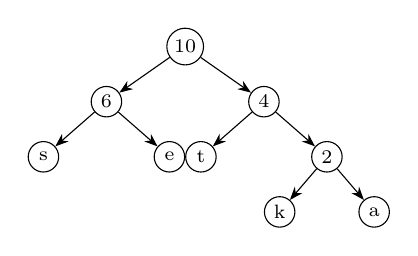
\begin{tikzpicture}[
    level distance=0.7cm,
    sibling distance=1.6cm,
    every node/.style={
        circle,
        draw,
        inner sep=1.5pt,
        minimum size=11pt,
        font=\scriptsize
    },
    edge from parent/.style={draw,-Stealth,thin},
    level 1/.style={sibling distance=2.0cm},
    level 2/.style={sibling distance=1.6cm},
    level 3/.style={sibling distance=1.2cm}
]
\node {10}
  child { node {6}
    child { node {s} }
    child { node {e} }
  }
  child { node {4}
    child { node {t} }
    child { node {2}
      child { node {k} }
      child { node {a} }
    }
  };
\end{tikzpicture}%
}
\end{center}
\vspace{-4pt}

\noindent
Frekvenstabell:$s:3, e:3, t:2, k:1, a:1$. Det er mange mulige Huffman-trær. Ulike trær gir ulik kode, men alle muligheter gir like mange bits for «s», like mange for «e», osv. Ett mulig valg av koder er for eksempel: $s:00, e:01,t:10,k:110, a:111.$ Her er «s», «e», «t» to-bits, mens «k» og «a» er tre-bits. Ordet «settekasse» kodes da som:
$\texttt{0001101001110111000001}$ som er 22 bits totalt.
\noindent
\textcolor{accentteal}{\textbf{Kan vi bruke dynamisk programmering for å lage en enkel og effektiv sorting algoritme?}}\\
Nei, dynamisk programmering hjelper når vi deler opp et stort problem, for å løse samme delproblene flere ganger da vi lagrer løsningene. Sortering kan bruke splitt og hersk som flette og quick, men det er lite sannsynlig at vi ser på samme delproblemer flere ganger i sortering. Å sjekke om en deltabell matcher en tidligere sortert tabell vil ta mer tid enn det sorteringsarbeidet vi sparer.
\textcolor{accentteal}{\textbf{Pristilsynet vil ha oversikt over 10 000 dagligvarer. De vil ha varane i en hashtabell, så de kan slå opp via pris. De vil for eksempel finne «alle varer som koster 200 kr» for å sjekke om butikkene følger regelverket. Tilsvarende for alle andre priser. Mange varer har priser som ender i enten 0 eller 9. Foreslå tabellstørrelse, hashfunksjon og kollisjonshåndtering så dette blir effektivt}}\color{black}. Det nevnes å finne alle varer med samme pris. Da er kollisjonshåndtering med \textbf{lenka lister} praktisk. Varer med samme pris hasher til samme sted, og havner på samme liste. Multiplikativ hashfunksjon kan brukes uten føringer for tabellstørrelse, når vi bruker lenka lister. Restdivisjon kan brukes, da er det en fordel å dele med et primtall (eller ihvertfall noe som ikke er tierpotens, siden mange priser ender på samme tall.) Tabellen bør vare stor nok til at ulike priser sjelden kolliderer. Det står ikke nok i oppgaven om hvor mange like priser det er, men om lag 10 000 vil vel være brukbart. Noe mindre, hvis det er mange like priser. For restdivisjon velger man et litt større primtall. \textbf{Åpen adressering} er også en mulighet. Da trenger vi et overhead på 20\% for å få god ytelse. Tabellstørrelsen bør altså være 12 000 eller mer. Åpen adressering med \textbf{restdivisjon}: Tabellstørrelse blir første primtall etter 12 000. Første hashfunksjon blir restdivisjon med tabellstørrelsen, andre hashfunksjon blir restdivisjon med (tabellstørrelse-1), hvor vi deretter legger til 1 for å unngå 0. Restdivisjon med mindre tall kan også brukes, fordi kortere hopp kan være bedre for cache. Åpen adressering med \textbf{multiplikativ hash}: alle tabellstørrelser kan brukes, men hashfunk- sjon nr 2 kan stille krav til tabellstørrelsen. Divisjonsbaserte funksjoner vil ofte kreve en primtallstørrelse. Eventuelt kan man gå for rask heltallsbasert multiplikativ hash, tabell- størrelse som er en toerpotens (16384), og oddetallsfunksjonen som hashfunksjon nr 2.
\color{accentteal}\textbf{Tellesortering egner seg ikke for desimaltall (float/double). Hvorfor ikke?~}\color{black}
Tellesortering bruker tallene som indeks i en tabell. Det fungerer ikke med desimaltall: 5,4 og 5,3 er ulike, men vil velge samme posisjon i tabellen likevel. De kan dermed komme ut i feil rekkefølge.
\textcolor{accentteal}{\textbf{Sett disse tallene (5,7,1,0,8,6,2) inn i en max-heap. Tegn opp hvordan heapen ser ut etter hvert tall.}}\\
\includegraphics[width=5cm]{images/maksheap.png}
\textcolor{accentteal}{\textbf{Sett de samme tallene inn i ett binært søketre. Tegn opp hvordan treet ser ut etter hvert tall}}\\
\includegraphics[height=1cm]{images/bintreoppg.png}
\textcolor{accentteal}{\textbf{Jeg trenger å lagre folkeregisteret for Norge i en hashtabell. Det er ca. 6 millioner personer. Personer skal kunne slåes opp på navn. Bruke dobbel hashing.}}
\textcolor{warmamber}{For å hashe navn, må de konverteres til tall på noe vis. Foreslå hvordan det kan gjøres i dette tilfellet.}Navn kan konverteres til tall med utgangspunkt i bokstavene. Deres unicodeverdier er tall. En veid sum blir et tall som kan brukes. Her bør vi vekte slik at alle tegn har effekt (ingen vektes med 0). Videre bør de vektes ulikt, så «Tri-Le» og «Le-Tri» ikke kolliderer. Til slutt må vi ha nok spredning, så de veide summene generelt blir større enn størrelsen på hashtabellen. En enkel og grei måte er å ta første tegn inn i en sum. Så ganger vi summen med et tall 13 (primtall, lite og ikke toerpotens), og legger til neste tegn. Slik fortsetter vi, gange med 13 og legge til neste, til alle tegnene er brukt opp. Vi får store tall, og ulik vekting av bokstavene.
\textcolor{warmamber}{Foreslå en størrelse på hashtabellen, og passende hashfunksjoner. Begrunn valgene du gjør.}
Vi ønsker plass til 6 mill. Generelt overhead er på ca. 20\%, så tabellstørrelsen bør være ca. 7,2 mill. To løsninger:
1. \textbf{Første løsning}, basert på restdivisjon. La $m$ være første primtall etter 7,2 mill. Hashfunksjonene blir $h_1(k)=k~mod~m$, $h_2(k)= k~mod~(m-1)+1$. Evt kan man bruke $h_2(k)= k~mod~7$ eller et lignende lavt tall, i håp om å dra nytte av caching når kollisjonskjeden ikke spres så mye. $h_2$ bør ha mer spredning enn forventet antall kollisjoner per innsetting. \textbf{Begrunnelser:} $h_1$ sprer over hele tabellen. $h_2$ får ingen felles faktorer med $m$, $h_2$ gir mindre tall enn primtallet $m$. $h_2$ blir heller ikke $0$. Tall som kolliderer i $h_1$, behøver ikke kollidere i $h_2$ også. 2. \textbf{Andre løsning}, multiplikativ hashfunksjon
La $t$ være første toerpotens etter 7,2 mill. $(2^3)$. Tabellstørrelsen blir $t$. Hashfunksjonene blir $h_1(k)=[t(kA-[kA])]$, $h_2=(2k+1)~mod~t$. Om en vil dra mer nytte av caching, kan en lavere toerpotens enn $t$ brukes i $h_2$, så lenge $h_2$ har mer spredning enn forventet antall kollisjoner. Med en toerpotens som tabellstørrelse, kan funksjonene implementeres med raske heltallsberegninger.
\textbf{Begrunnelser:} $h_1$ sprer over hele tabellen. $h_2$ lager oddetall, som ikke har felles faktorer med en toerpotens. Tall som kolliderer i $h_1$, behøver ikke kollidere i $h_2$ også.



%-------- skriv alt ^^
}
\end{multicols}
\end{document}
